\documentclass[]{article}
\usepackage{amsmath}
\usepackage{pdfpages}
%opening
\title{Formale Methoden- Übungsserie 5}
\author{Tobias Reincke \\ Matrikelnummer: 218203884}


\begin{document}

\maketitle



\section{Aufgabe 1}
\subsection{a}
Ja.
\subsection{b}
Nein. Dieses Zeichen ist kein Zustand, sondern eine Aktion.\\ $Prozess: Zustandsmenge \times Aktionsmenge \to Zustandsmenge  $
\subsection{c}
Ja.
\subsection{d}
Nein. (Es gibt eine Q.0, welches P nicht hat.)
\subsection{e}
Nein. Die Simulation von dem einen auf das andere, muss \underline{invers} zu das andere auf dem einen sein.
\subsection{f}
Ja, es ist eine Bedingung für Bisimularität.

\section{Aufgabe 2 }
\subsection{a}
$Tr(P) = \{P_m, P_{m.o},P_{m.o.n}, P_m, P _ {m.n}, P_{m.n.p} \}$ \\
$Tr(Q)= \{Q_{m}, Q_{m.o},Q_{m.o.n},Q_{m.n},Q_{m.n.p},Q_{m.n}                                                                                                                                          \}  $
\subsection{b}
$CT(P)= \{            P_{m.o.n},      P_{m.n.p}                                                                                    \}    $\\
$CT(Q)= \{                Q_{m.o.n},Q_{m.n},Q_{m.n.p}                                                                                              \}$

\subsection{c}
Die Bedingung  für Traceäquivalenz ist, dass die Menge der Traces übereinstimmen. Das ist hier der Fall. 
\subsection{d}
Nein. $Q_{m.n}$ ist in Q vollständig, aber in P nicht.
\subsection{ e}
Ja, alle vollstandigen Traces in P gibt es auch in Q. \\
 $ \{ P_{m.o.n},      P_{m.n.p} \} =  \{ Q_{m.o.n},      Q_{m.n.p}                                                 \}\subseteq CT(Q)      $
 \section{Aufgabe 3}
 
 \textit{$P := q.(0 | r.0)  \\ Q:= q.r.0  $ }
 \subsection{a}
 Ja. $P - q\rightarrow P^{'} , Q-q \rightarrow Q^{'} \land P^{'} -r \rightarrow P^{''} , Q^{'}-r  \rightarrow Q^{''} \longrightarrow PsQ \land P^{'}s Q^{'} $
 
 \subsection{b}
 Nein. Es gibt den Entscheidungsfall nicht, dass im rechte Teilbaum, dass r ausgeführt werden kann.
 
 \subsection{c}
 Nein: P simuliert  Q, Q simuliert aber P nicht.

 \section{Aufgabe 4}

 \includepdf[pages=2]{Zeichnung rofl.pdf}



\end{document}
